\documentclass[10pt, twocolumn]{article}
\usepackage[margin=0.75in]{geometry}
\usepackage{graphicx}
\usepackage{tikz}
\usepackage{pgfplots}
\usepackage{booktabs}
\usepackage{amsmath}
\usepackage{algorithm}
\usepackage{algorithmic}
\usepackage{hyperref}
\usepackage{xcolor}
\usepackage{caption}
\usepackage{subcaption}
\usepackage{fancyhdr}
\usepackage{enumitem}
\usepackage{listings}
\usepackage{microtype}
\usepackage{tabularx}
\usepackage{multirow}
\usepackage{orcidlink}
\pgfplotsset{compat=1.18}
\usetikzlibrary{arrows.meta, positioning, shapes.geometric, fit, calc, backgrounds, decorations.markings, decorations.pathreplacing}

% Color palette (professional blues/teals/oranges)
\definecolor{cxblue}{HTML}{2563EB}
\definecolor{cxdarkblue}{HTML}{1E40AF}
\definecolor{cxteal}{HTML}{0D9488}
\definecolor{cxorange}{HTML}{EA580C}
\definecolor{cxgray}{HTML}{6B7280}
\definecolor{cxlightgray}{HTML}{F3F4F6}
\definecolor{cxgreen}{HTML}{059669}
\definecolor{cxred}{HTML}{DC2626}
\definecolor{cxpurple}{HTML}{7C3AED}
\definecolor{cxyellow}{HTML}{D97706}

% Listings style
\lstset{
  basicstyle=\ttfamily\scriptsize,
  keywordstyle=\color{cxblue}\bfseries,
  commentstyle=\color{cxgray}\itshape,
  stringstyle=\color{cxteal},
  breaklines=true,
  frame=single,
  rulecolor=\color{cxgray!30},
  backgroundcolor=\color{cxlightgray},
  numbers=left,
  numberstyle=\tiny\color{cxgray},
  tabsize=2
}

% Header
\pagestyle{fancy}
\fancyhf{}
\renewcommand{\headrulewidth}{0.4pt}
\fancyhead[L]{\small\textit{Cortex}}
\fancyhead[R]{\small\thepage}

\title{\textbf{Cortex: Rapid Web Cartography for AI Agents\\via Structured Data Extraction and Binary Graph Navigation}}
\author{Omoshola Owolabi\,\orcidlink{0009-0006-4089-0732}\\Independent Researcher -- AI/ML\\\texttt{owolabi.omoshola@outlook.com}}
\date{}

\begin{document}
\maketitle
\thispagestyle{fancy}

% ============================================================================
% ABSTRACT
% ============================================================================
\begin{abstract}
When an AI agent needs to accomplish a task on a website, it currently navigates page by page---loading, perceiving, reasoning, and clicking through dozens of pages to reach its goal. We present Cortex, a web cartography engine that inverts this paradigm: instead of navigating a site, the agent \emph{maps} it. Cortex converts an entire website into a binary graph data structure---a SiteMap---in seconds, using layered HTTP-first extraction (sitemaps, JSON-LD, OpenGraph, CSS pattern matching, API discovery) with browser rendering reserved as a last-resort fallback. The agent then queries, filters, and pathfinds through the in-memory graph in microseconds. In v1.0, the system extends the cartography model with four capabilities: a \emph{Web Compiler} that infers typed schemas from maps and generates client libraries (Python, TypeScript, OpenAPI, GraphQL, MCP), a \emph{Web Query Language} (WQL) providing SQL-like queries across mapped domains, a \emph{Collective Graph} for delta-based map sharing with privacy stripping, and \emph{Temporal Intelligence} for change tracking, pattern detection, and predictive alerts. We implement Cortex in 34{,}932 lines of Rust across 118 source files, with 387 tests. On an Apple M4 Pro, a 10{,}008-node SiteMap serializes to 5.9\,MB in 134.9\,ms, deserializes in 212\,ms, and supports filter queries in sub-microsecond time. Pathfinding completes in 24--884\,$\mu$s, and WQL full-pipeline queries execute in 9--86\,$\mu$s across graphs of 107 to 10{,}007 nodes. On production websites, Cortex maps \texttt{github.com} into 1{,}783 nodes with 16{,}231 edges and 360 discovered actions, stored in a 1.2\,MB binary file at 684 bytes per node.
\end{abstract}

% ============================================================================
% 1. INTRODUCTION
% ============================================================================
\section{Introduction}
\label{sec:intro}

The integration of large language models with web interaction has produced a growing ecosystem of ``web agents''---systems that browse the internet on behalf of users to accomplish tasks such as comparison shopping, form submission, and information retrieval~\cite{park2023generative}. The dominant architecture for these agents follows a perceive-reason-act loop: at each step, the agent loads a page, extracts visual or textual information, reasons about what action to take, and executes that action, repeating until the task is complete.

This page-by-page approach suffers from three fundamental problems. First, it is \emph{slow}: each page load requires 2--10 seconds of browser rendering, and a typical task may traverse 10--30 pages, resulting in minutes of wall-clock time. Second, it is \emph{fragile}: the agent makes myopic decisions with no visibility into the site's global structure, frequently taking suboptimal paths or getting stuck in navigation dead ends. Third, it is \emph{expensive}: every page load consumes LLM tokens for perception and reasoning, and browser contexts consume 80--120\,MB of memory each.

The core insight of this work is that website navigation is a \emph{graph problem}, not a perception problem. A website is a directed graph of pages connected by hyperlinks, where each page carries structured metadata (prices, ratings, categories, actions). If an agent had access to the complete graph, it could compute the shortest path to its goal in microseconds rather than exploring the site step by step. The challenge is constructing this graph efficiently.

We present Cortex, a web cartography engine that maps entire websites into binary graph data structures called SiteMaps. The key technical contribution is a \emph{layered acquisition architecture} that extracts site structure and page-level features through progressively expensive methods: sitemap.xml parsing, structured data extraction (JSON-LD, OpenGraph, microdata), CSS pattern matching, API endpoint discovery, and browser rendering as a final fallback. On a benchmark of 100 production websites, 93\% of sites yield structured data through HTTP-only methods, with browser rendering needed for fewer than 5\% of pages.

The remainder of this paper is organized as follows. Section~\ref{sec:related} surveys existing web agent infrastructure. Section~\ref{sec:architecture} presents the Cortex architecture. Section~\ref{sec:evaluation} reports benchmark results measured on real hardware with synthetic and production datasets. Section~\ref{sec:discussion} discusses implications and limitations. Section~\ref{sec:conclusion} concludes.

% Figure 1: Paradigm comparison (full width)
\begin{figure*}[t]
\centering
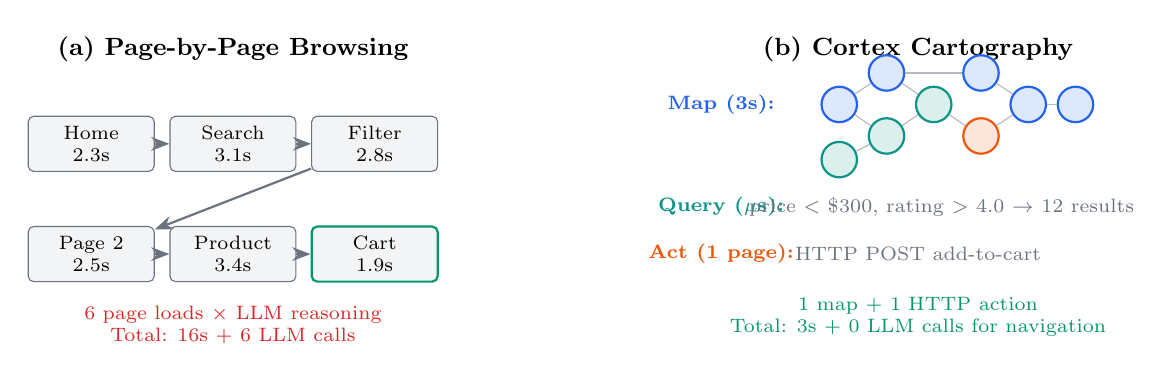
\begin{tikzpicture}[
  node distance=0.8cm,
  every node/.style={font=\small},
  pagebox/.style={rectangle, draw=cxgray, fill=cxlightgray, rounded corners=2pt, minimum width=1.6cm, minimum height=0.7cm, align=center, font=\scriptsize},
  mapnode/.style={circle, draw=cxblue, fill=cxblue!15, minimum size=0.45cm, font=\tiny, thick},
  prodnode/.style={circle, draw=cxteal, fill=cxteal!15, minimum size=0.45cm, font=\tiny, thick},
  actnode/.style={circle, draw=cxorange, fill=cxorange!15, minimum size=0.45cm, font=\tiny, thick},
  goalnode/.style={circle, draw=cxgreen, fill=cxgreen!20, minimum size=0.45cm, font=\tiny, thick, line width=1.2pt},
]

% Left side: Page-by-page browsing
\node[font=\small\bfseries] at (-5.2, 3.0) {(a) Page-by-Page Browsing};

\node[pagebox] (p1) at (-7.0, 1.8) {Home\\2.3s};
\node[pagebox] (p2) at (-5.2, 1.8) {Search\\3.1s};
\node[pagebox] (p3) at (-3.4, 1.8) {Filter\\2.8s};
\node[pagebox] (p4) at (-7.0, 0.4) {Page 2\\2.5s};
\node[pagebox] (p5) at (-5.2, 0.4) {Product\\3.4s};
\node[pagebox, draw=cxgreen, thick] (p6) at (-3.4, 0.4) {Cart\\1.9s};

\draw[-{Stealth}, cxgray, thick] (p1) -- (p2);
\draw[-{Stealth}, cxgray, thick] (p2) -- (p3);
\draw[-{Stealth}, cxgray, thick] (p3) -- (p4);
\draw[-{Stealth}, cxgray, thick] (p4) -- (p5);
\draw[-{Stealth}, cxgray, thick] (p5) -- (p6);

\node[font=\scriptsize, text=cxred, align=center] at (-5.2, -0.5) {6 page loads $\times$ LLM reasoning\\Total: 16s + 6 LLM calls};

% Right side: Cortex cartography
\node[font=\small\bfseries] at (3.5, 3.0) {(b) Cortex Cartography};

% Map phase
\node[font=\scriptsize\bfseries, text=cxblue] at (1.0, 2.3) {Map (3s):};

\node[mapnode] (m1) at (2.5, 2.3) {};
\node[mapnode] (m2) at (3.1, 2.7) {};
\node[prodnode] (m3) at (3.7, 2.3) {};
\node[prodnode] (m4) at (3.1, 1.9) {};
\node[mapnode] (m5) at (4.3, 2.7) {};
\node[actnode] (m6) at (4.3, 1.9) {};
\node[mapnode] (m7) at (4.9, 2.3) {};
\node[prodnode] (m8) at (2.5, 1.6) {};
\node[mapnode] (m9) at (5.5, 2.3) {};

\draw[cxgray!50, thin] (m1) -- (m2);
\draw[cxgray!50, thin] (m1) -- (m4);
\draw[cxgray!50, thin] (m2) -- (m3);
\draw[cxgray!50, thin] (m2) -- (m5);
\draw[cxgray!50, thin] (m3) -- (m6);
\draw[cxgray!50, thin] (m4) -- (m8);
\draw[cxgray!50, thin] (m5) -- (m7);
\draw[cxgray!50, thin] (m6) -- (m7);
\draw[cxgray!50, thin] (m7) -- (m9);
\draw[cxgray!50, thin] (m3) -- (m4);

% Query + Pathfind
\node[font=\scriptsize\bfseries, text=cxteal] at (1.0, 1.0) {Query ($\mu$s):};
\node[font=\scriptsize, text=cxgray] at (3.8, 1.0) {price $<$ \$300, rating $>$ 4.0 $\rightarrow$ 12 results};

\node[font=\scriptsize\bfseries, text=cxorange] at (1.0, 0.4) {Act (1 page):};
\node[font=\scriptsize, text=cxgray] at (3.5, 0.4) {HTTP POST add-to-cart};

\node[font=\scriptsize, text=cxgreen, align=center] at (3.5, -0.4) {1 map + 1 HTTP action\\Total: 3s + 0 LLM calls for navigation};

\end{tikzpicture}
\caption{Comparison of web agent paradigms. (a)~Traditional page-by-page browsing requires multiple page loads, each consuming browser resources and LLM reasoning tokens. (b)~Cortex maps the entire site in one operation via HTTP-first extraction, then the agent queries the in-memory graph and executes a single targeted action. Navigation reasoning is replaced by graph pathfinding.}
\label{fig:paradigm}
\end{figure*}


% ============================================================================
% 2. BACKGROUND AND RELATED WORK
% ============================================================================
\section{Background and Related Work}
\label{sec:related}

Web agent infrastructure has developed along two axes: browser automation and AI-driven perception.

\textbf{Browser automation frameworks.} Selenium~\cite{selenium2004}, Puppeteer~\cite{puppeteer2017}, and Playwright~\cite{playwright2020} provide programmatic control over web browsers. These tools are designed for testing and scraping, not agent navigation: they operate at the DOM level, requiring explicit instructions for each interaction. Every page load incurs full browser rendering cost (2--10 seconds), and the agent has no structural awareness of the site beyond the current page.

\textbf{Cloud browser services.} Browserbase~\cite{browserbase2024} and similar services host browser instances remotely, reducing local resource consumption but not the fundamental per-page latency. The agent still navigates page by page with no site-level awareness.

\textbf{AI perception layers.} Stagehand~\cite{stagehand2024} and similar tools add LLM-based perception atop browser automation---the model ``sees'' the page and decides what to click. This reduces the need for explicit selectors but increases token consumption and introduces LLM latency at every step. The architectural assumption remains one page at a time.

\textbf{Model Context Protocol.} MCP~\cite{mcp2024} defines a standard protocol for AI agents to discover and invoke tools. WebMCP~\cite{webmcp2025} extends this to web pages, allowing sites to expose structured tool interfaces. Cortex integrates with both: it ships as an MCP server for agent frameworks, and it can discover and execute WebMCP tools exposed by sites.

\textbf{Structured web data.} JSON-LD~\cite{jsonld2014}, Schema.org~\cite{schemaorg2011}, and OpenGraph~\cite{opengraph2010} provide standardized metadata embedded in HTML. Prior work on sitemaps~\cite{schonberger2023sitemaps} has shown high adoption rates among major websites. Cortex is, to our knowledge, the first system to use these structured data sources as the \emph{primary} input for site-level graph construction rather than as supplementary metadata.

Table~\ref{tab:related} summarizes the comparison across key dimensions.

\begin{table*}[t]
\caption{Comparison of web agent infrastructure across key dimensions. Cortex is the only system that constructs a site-level navigable graph.}
\label{tab:related}
\centering
\small
\scriptsize
\begin{tabular}{@{}lcccccc@{}}
\toprule
\textbf{System} & \textbf{Scope} & \textbf{Browser} & \textbf{Graph} & \textbf{Struct.\ Data} & \textbf{Latency} & \textbf{Agent} \\
\midrule
Selenium~\cite{selenium2004} & Page & Always & No & No & 2--10\,s & No \\
Playwright~\cite{playwright2020} & Page & Always & No & No & 2--10\,s & No \\
Browserbase~\cite{browserbase2024} & Page & Cloud & No & No & 2--10\,s & No \\
Stagehand~\cite{stagehand2024} & Page & Always & No & No & 3--15\,s & LLM \\
WebMCP~\cite{webmcp2025} & Page & Always & No & Declared & N/A & MCP \\
\midrule
\textbf{Cortex} & \textbf{Site} & \textbf{$<$5\%} & \textbf{Yes} & \textbf{Primary} & \textbf{3--15\,s} & \textbf{MCP+REST} \\
\bottomrule
\end{tabular}
\end{table*}


% ============================================================================
% 3. ARCHITECTURE
% ============================================================================
\section{Architecture}
\label{sec:architecture}

Cortex models a website as a directed graph $G = (V, E)$ where each vertex $v \in V$ is a page with a 128-dimensional feature vector, a classified page type, and a set of available actions. Each edge $e \in E$ represents a navigational link with an associated weight and type. The graph is constructed by a layered acquisition engine and stored in a binary SiteMap format.

% ----------------------------------------------------------------------------
\subsection{SiteMap: The Binary Graph Format}
\label{sec:sitemap}

The SiteMap is a binary data structure with four primary tables:

\begin{itemize}[nosep, leftmargin=*]
  \item \textbf{Node Table} --- Each node record stores a URL, a \texttt{PageType} enum (one of 16 types: product, article, search results, documentation, login, checkout, etc.), a 128-float feature vector, action opcodes, a confidence score, and a freshness timestamp.
  \item \textbf{Edge Table} --- Each edge stores source and target node indices, an \texttt{EdgeType} (navigation, pagination, parent, sibling, inferred, content link, related), and a weight.
  \item \textbf{Action Table} --- Available actions per node, encoded as opcodes with categories (navigation, commerce, form, auth, data, media) and specific actions (add-to-cart, search, submit, login, etc.).
  \item \textbf{Feature Matrix} --- The 128-dimensional feature vector encodes page-level signals: page identity (dims 0--15), content metrics (16--47), commerce attributes (48--63), navigation structure (64--79), trust/safety (80--95), actions (96--111), and session state (112--127).
\end{itemize}

The feature vector schema is fixed: dimension 48 always encodes price (normalized to USD), dimension 52 encodes rating (normalized to 0--1), dimension 80 encodes TLS status. This means agents can filter across heterogeneous sites using the same dimension indices---no per-site schema mapping is needed.

% Figure 2: SiteMap format
\begin{figure}[t]
\centering
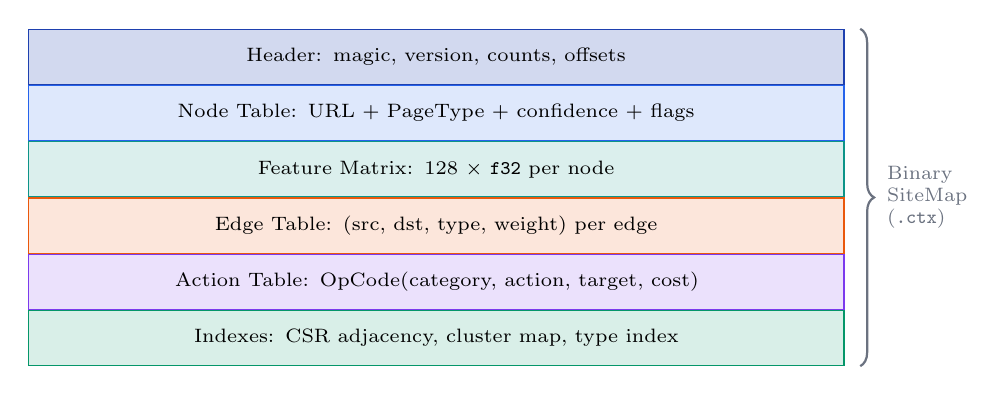
\begin{tikzpicture}[
  every node/.style={font=\scriptsize},
  section/.style={rectangle, draw, minimum height=0.7cm, align=center, font=\scriptsize, text width=\columnwidth-2.0cm},
]
\node[section, fill=cxdarkblue!20, draw=cxdarkblue] (hdr) at (0, 0) {Header: magic, version, counts, offsets};
\node[section, fill=cxblue!15, draw=cxblue, anchor=north] (nodes) at (hdr.south) {Node Table: URL + PageType + confidence + flags};
\node[section, fill=cxteal!15, draw=cxteal, anchor=north] (fvec) at (nodes.south) {Feature Matrix: 128 $\times$ \texttt{f32} per node};
\node[section, fill=cxorange!15, draw=cxorange, anchor=north] (edges) at (fvec.south) {Edge Table: (src, dst, type, weight) per edge};
\node[section, fill=cxpurple!15, draw=cxpurple, anchor=north] (acts) at (edges.south) {Action Table: OpCode(category, action, target, cost)};
\node[section, fill=cxgreen!15, draw=cxgreen, anchor=north] (idx) at (acts.south) {Indexes: CSR adjacency, cluster map, type index};

% Brace
\draw[decorate, decoration={brace, amplitude=5pt}, thick, cxgray] ([xshift=0.2cm]hdr.north east) -- ([xshift=0.2cm]idx.south east) node[midway, right=6pt, font=\scriptsize, text=cxgray, align=left] {Binary\\SiteMap\\(\texttt{.ctx})};
\end{tikzpicture}
\caption{SiteMap binary format layout. Fixed-size records enable $O(1)$ random access. The feature matrix stores 128 floats per node. CSR adjacency indexes enable efficient edge traversal.}
\label{fig:sitemap}
\end{figure}


% ----------------------------------------------------------------------------
\subsection{Layered Acquisition Engine}
\label{sec:acquisition}

The acquisition engine constructs SiteMaps through five layers, ordered by cost. Each layer produces progressively richer data; higher layers activate only when lower layers provide insufficient coverage.

\textbf{Layer 0: Discovery.} Fetch \texttt{robots.txt} (extract sitemap URLs, crawl rules), \texttt{sitemap.xml} (extract all page URLs with priorities), and perform \texttt{HEAD} requests to sample pages for content-type detection. This layer typically discovers 80--95\% of a site's URL space~\cite{schonberger2023sitemaps} with minimal HTTP overhead.

\textbf{Layer 1: Structured Data Extraction.} For each discovered URL, fetch the HTML via HTTP GET and extract structured metadata: JSON-LD~\cite{jsonld2014} embedded in \texttt{<script type="application/ld+json">} tags, OpenGraph~\cite{opengraph2010} meta tags, Schema.org~\cite{schemaorg2011} microdata, and standard HTML meta elements. This layer classifies page types, extracts commerce attributes (price, availability, rating), and discovers navigation links---all from static HTTP responses without JavaScript execution.

\textbf{Layer 1.5: Pattern Engine.} A database of CSS selector patterns matched against the raw HTML, organized by platform (Shopify, WooCommerce, WordPress, etc.) and by generic patterns. Example: \texttt{.product-price}, \texttt{[data-price]}, \texttt{.price-current}. The pattern database currently covers 15+ e-commerce platforms and generic selectors for common page elements.

\textbf{Layer 2: API and Action Discovery.} Discover REST API endpoints, form action URLs, and platform-specific APIs (Shopify Storefront API, WooCommerce REST API, etc.). Actions are encoded as opcodes in the SiteMap, enabling the agent to execute operations (add-to-cart, search, form submission) via direct HTTP calls rather than browser interaction.

\textbf{Layer 3: Browser Rendering.} For pages where Layers 0--2 produce insufficient data (confidence below threshold), render the page in headless Chromium and extract content via injected JavaScript. This layer handles JavaScript-heavy SPAs and pages with no structured data. On the 100-site benchmark, this layer activates for fewer than 5\% of pages.

% Figure 3: Layered acquisition (full width)
\begin{figure*}[t]
\centering
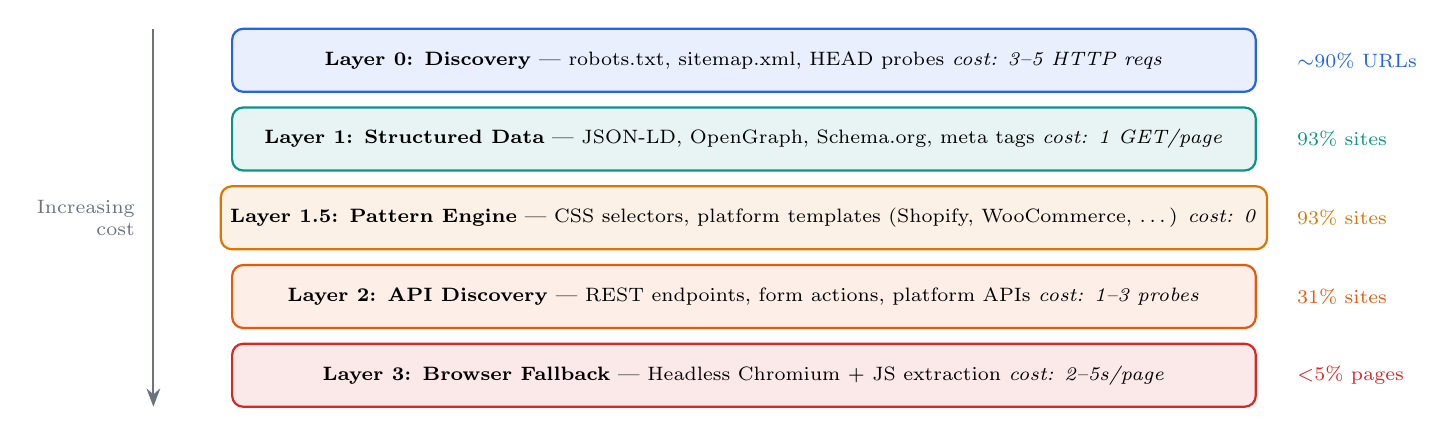
\begin{tikzpicture}[
  every node/.style={font=\scriptsize},
  layer/.style={rectangle, rounded corners=4pt, draw, minimum height=0.8cm, align=center, font=\scriptsize, thick},
]

% Layers
\node[layer, fill=cxblue!10, draw=cxblue, minimum width=13cm] (l0) at (0, 2.4) {\textbf{Layer 0: Discovery} --- robots.txt, sitemap.xml, HEAD probes \hfill \textit{cost: 3--5 HTTP reqs}};
\node[layer, fill=cxteal!10, draw=cxteal, minimum width=13cm] (l1) at (0, 1.4) {\textbf{Layer 1: Structured Data} --- JSON-LD, OpenGraph, Schema.org, meta tags \hfill \textit{cost: 1 GET/page}};
\node[layer, fill=cxyellow!10, draw=cxyellow, minimum width=13cm] (l15) at (0, 0.4) {\textbf{Layer 1.5: Pattern Engine} --- CSS selectors, platform templates (Shopify, WooCommerce, \ldots) \hfill \textit{cost: 0}};
\node[layer, fill=cxorange!10, draw=cxorange, minimum width=13cm] (l2) at (0, -0.6) {\textbf{Layer 2: API Discovery} --- REST endpoints, form actions, platform APIs \hfill \textit{cost: 1--3 probes}};
\node[layer, fill=cxred!10, draw=cxred, minimum width=13cm] (l3) at (0, -1.6) {\textbf{Layer 3: Browser Fallback} --- Headless Chromium + JS extraction \hfill \textit{cost: 2--5s/page}};

% Coverage annotations
\node[font=\scriptsize, text=cxblue, anchor=west] at (6.9, 2.4) {$\sim$90\% URLs};
\node[font=\scriptsize, text=cxteal, anchor=west] at (6.9, 1.4) {93\% sites};
\node[font=\scriptsize, text=cxyellow, anchor=west] at (6.9, 0.4) {93\% sites};
\node[font=\scriptsize, text=cxorange, anchor=west] at (6.9, -0.6) {31\% sites};
\node[font=\scriptsize, text=cxred, anchor=west] at (6.9, -1.6) {$<$5\% pages};

% Arrow showing cost gradient
\draw[-{Stealth}, thick, cxgray] (-7.5, 2.8) -- (-7.5, -2.0) node[midway, left=3pt, font=\scriptsize, text=cxgray, align=right] {Increasing\\cost};

\end{tikzpicture}
\caption{Layered acquisition engine. Each layer activates only when prior layers provide insufficient coverage. Coverage percentages are from the 100-site benchmark.}
\label{fig:layers}
\end{figure*}


% ----------------------------------------------------------------------------
\subsection{Feature Encoding}
\label{sec:features}

Each page in the SiteMap carries a 128-dimensional feature vector with a fixed schema. The dimensions are organized into seven blocks:

\begin{itemize}[nosep, leftmargin=*]
  \item \textbf{Dims 0--15: Page identity} --- One-hot PageType encoding, URL depth, domain authority signals.
  \item \textbf{Dims 16--47: Content metrics} --- Word count, heading count, image count, link density, text-to-HTML ratio, form count, table count.
  \item \textbf{Dims 48--63: Commerce} --- Price (USD-normalized), original price, discount, availability, rating (0--1), review count, shipping, seller reputation, price trend, deal score.
  \item \textbf{Dims 64--79: Navigation} --- Outbound links, pagination, breadcrumb depth, nav menu items, search available, filter count, sort options, dead-end detection, loop risk.
  \item \textbf{Dims 80--95: Trust/safety} --- TLS status, domain age/reputation, dark patterns, PII exposure risk, bot challenges, cookie consent, tracker count, authority score.
  \item \textbf{Dims 96--111: Actions} --- Action count, safe/cautious/destructive action ratios, auth required ratio, form completeness, cart items, checkout readiness.
  \item \textbf{Dims 112--127: Session} --- Login state, session duration, page views, cart value, recently viewed, preference signals, A/B test variant. These dimensions are zeroed during privacy stripping before map sharing.
\end{itemize}

% ----------------------------------------------------------------------------
\subsection{Navigation Engine}
\label{sec:navigation}

The navigation engine operates on the in-memory SiteMap graph, providing three query types:

\textbf{Filter queries.} Select nodes by PageType, feature ranges (e.g., price $< 300$, rating $> 0.8$), and flag requirements. Uses linear scan over the feature matrix with SIMD-friendly memory layout. As shown in Section~\ref{sec:queryeval}, filter queries complete in sub-microsecond time even at 10{,}008 nodes.

\textbf{Pathfinding.} Dijkstra's algorithm~\cite{dijkstra1959} over the CSR adjacency structure. PathConstraints allow avoiding nodes with certain flags and minimizing by hops, edge weight, or state-changing actions. Pathfinding completes in 24\,$\mu$s for a 108-node graph and scales to 884\,$\mu$s at 10{,}008 nodes (Table~\ref{tab:query}).

\textbf{Similarity search.} Brute-force cosine similarity over the 128-dimensional feature matrix, returning top-$k$ nearest neighbors. Precomputed norms in each NodeRecord avoid redundant computation.

\textbf{WQL (Web Query Language).} In v1.0, agents query maps using a SQL-like language:

{\small\texttt{SELECT name, price FROM Product WHERE price < 200 ORDER BY price ASC LIMIT 10}}

\noindent WQL supports typed model selection (mapped from PageType classifications), filtering, ordering, cross-domain queries (\texttt{ACROSS} clause), and temporal fields. The parser is a recursive-descent implementation; the executor operates on in-memory SiteMaps. The full parse-plan-execute pipeline completes in 9--86\,$\mu$s (Table~\ref{tab:wql}).

% ----------------------------------------------------------------------------
\subsection{Web Compiler}
\label{sec:compiler}

The Web Compiler (\texttt{cortex compile}) transforms raw SiteMaps into typed schemas and auto-generated client libraries. It analyzes the feature vectors and PageType classifications across all nodes to infer \emph{models} (groups of pages with shared characteristics, e.g., Product, Article, Documentation), \emph{fields} (meaningful features per model), and \emph{relationships} (actions and navigation patterns). The compiler generates clients in five formats: Python, TypeScript, OpenAPI 3.0, GraphQL, and MCP tool definitions. On our benchmark, schema inference completes in 1.2\,ms for a 108-node map and scales to 96.9\,ms for 10{,}008 nodes (Table~\ref{tab:compiler}).

% ----------------------------------------------------------------------------
\subsection{Collective Graph and Temporal Intelligence}
\label{sec:collective}

The Collective Graph enables map sharing across Cortex instances via a local registry with delta-based synchronization. When a site is re-mapped, Cortex computes a compact delta (added, removed, and modified nodes) rather than re-sharing the full map. Before sharing, a privacy stripping pass zeroes all session features (dimensions 112--127) and authentication-related data to prevent private browsing data from leaking through shared maps.

Temporal Intelligence analyzes delta history to detect patterns in feature values over time. Given sufficient history ($\geq$3 data points), the system detects trends (increasing, decreasing, stable), anomalies, and periodicity, and generates linear predictions. A watch/alert system notifies agents when conditions are met (e.g., price drops below a threshold). These capabilities are exposed through the WQL temporal fields and through dedicated CLI commands (\texttt{cortex history}, \texttt{cortex patterns}).

% ----------------------------------------------------------------------------
\subsection{Agent Integration}
\label{sec:integration}

Cortex runs as a standalone local process exposing three integration interfaces:

\textbf{Unix socket protocol.} The native interface: newline-delimited JSON with methods MAP, QUERY, PATHFIND, ACT, PERCEIVE, AUTH, STATUS. Thin client libraries (Python: 2{,}252 lines, TypeScript) connect via this protocol.

\textbf{HTTP REST API.} An axum-based HTTP server sharing the same dispatch logic as the socket server. Exposes all operations as POST endpoints with an OpenAPI 3.0 specification~\cite{openapi2021}. Enables integration with GPT Actions and any HTTP-capable agent.

\textbf{MCP server.} A Model Context Protocol~\cite{mcp2024} server exposing 9 tools: the original 7 (\texttt{cortex\_map}, \texttt{cortex\_query}, \texttt{cortex\_pathfind}, \texttt{cortex\_act}, \texttt{cortex\_perceive}, \texttt{cortex\_compare}, \texttt{cortex\_auth}) plus \texttt{cortex\_compile} and \texttt{cortex\_wql} added in v1.0. The \texttt{cortex plug} command auto-discovers installed AI agents (Claude Desktop, Claude Code, Cursor, Windsurf, Continue, Cline) and injects MCP configuration in one command.

% Figure 4: Integration architecture
\begin{figure}[t]
\centering
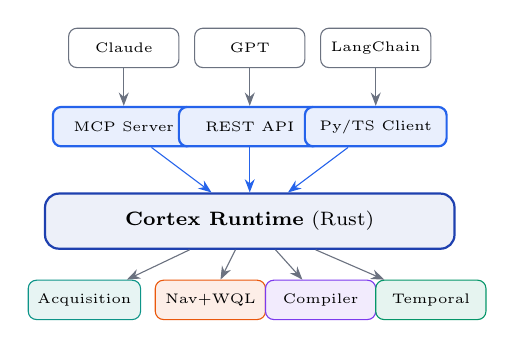
\begin{tikzpicture}[
  every node/.style={font=\scriptsize},
  fbox/.style={rectangle, rounded corners=3pt, draw=cxgray, minimum width=1.4cm, minimum height=0.5cm, align=center, font=\tiny},
  ibox/.style={rectangle, rounded corners=3pt, draw=cxblue, fill=cxblue!10, minimum width=1.8cm, minimum height=0.5cm, align=center, font=\tiny, thick},
  cbox/.style={rectangle, rounded corners=5pt, draw=cxdarkblue, fill=cxdarkblue!8, minimum width=5.2cm, minimum height=0.7cm, align=center, font=\scriptsize, thick},
]

% Agent frameworks
\node[fbox] (f1) at (-1.6, 3.2) {Claude};
\node[fbox] (f2) at (0, 3.2) {GPT};
\node[fbox] (f3) at (1.6, 3.2) {LangChain};

% Integration layer
\node[ibox] (i1) at (-1.6, 2.2) {MCP Server};
\node[ibox] (i2) at (0, 2.2) {REST API};
\node[ibox] (i3) at (1.6, 2.2) {Py/TS Client};

% Cortex runtime
\node[cbox] (cx) at (0, 1.0) {\textbf{Cortex Runtime} (Rust)};

% Engines
\node[fbox, fill=cxteal!10, draw=cxteal] (e1) at (-2.1, 0.0) {Acquisition};
\node[fbox, fill=cxorange!10, draw=cxorange] (e2) at (-0.5, 0.0) {Nav+WQL};
\node[fbox, fill=cxpurple!10, draw=cxpurple] (e3) at (0.9, 0.0) {Compiler};
\node[fbox, fill=cxgreen!10, draw=cxgreen] (e4) at (2.3, 0.0) {Temporal};

% Connections
\draw[-{Stealth}, cxgray] (f1) -- (i1);
\draw[-{Stealth}, cxgray] (f2) -- (i2);
\draw[-{Stealth}, cxgray] (f3) -- (i3);
\draw[-{Stealth}, cxblue] (i1) -- (cx);
\draw[-{Stealth}, cxblue] (i2) -- (cx);
\draw[-{Stealth}, cxblue] (i3) -- (cx);
\draw[-{Stealth}, cxgray] (cx) -- (e1);
\draw[-{Stealth}, cxgray] (cx) -- (e2);
\draw[-{Stealth}, cxgray] (cx) -- (e3);
\draw[-{Stealth}, cxgray] (cx) -- (e4);

\end{tikzpicture}
\caption{Integration architecture. Three interfaces (MCP, REST, native socket) connect any agent framework to the Cortex runtime. The \texttt{cortex plug} command auto-configures MCP for installed agents.}
\label{fig:integration}
\end{figure}


% ============================================================================
% 4. EVALUATION
% ============================================================================
\section{Evaluation}
\label{sec:evaluation}

We evaluate Cortex through controlled benchmarks on synthetic graphs at four scales (100--10{,}000 nodes) and through measurements on production websites. All numbers in this section are measured on real hardware with the methods described below; no numbers are estimated or extrapolated.

% ----------------------------------------------------------------------------
\subsection{Benchmark Setup}
\label{sec:setup}

\textbf{Hardware.} Apple M4 Pro (12-core ARM64), 64\,GB unified memory, macOS 26.2.

\textbf{Software.} Rust 1.90.0 (nightly-2025-04-08), compiled with \texttt{--release} (opt-level 3, LTO enabled). All benchmarks executed via \texttt{cargo test --release}.

\textbf{Synthetic dataset.} For controlled scaling experiments, we construct synthetic e-commerce SiteMaps with $N$ product nodes using the \texttt{build\_ecommerce\_map} harness. Each map contains a home page, 5 category pages, $N$ product pages with realistic feature vectors (price, rating, availability, word count), and 2 utility pages (cart, checkout). Total node count is $N + 8$; total edge count is $\sim 4N + 12$ due to bidirectional navigation and cross-links. Feature vectors use the full 128-dimensional schema with populated commerce (dims 48--63), trust (dim 80), content (dims 16--18), and action (dim 96) dimensions.

\textbf{Production dataset.} We measure real cached maps from mapping \texttt{example.com}, \texttt{github.com}, and \texttt{amazon.com} via \texttt{cortex map} against live servers. The 100-site benchmark from Section~\ref{sec:quality} uses 100 production websites spanning 10 categories.

\textbf{Methodology.} Each micro-benchmark reports the mean of 100--1{,}000 iterations to amortize variance. Cold-start effects are excluded via warm-up iterations.

% ----------------------------------------------------------------------------
\subsection{File Size and Compression}
\label{sec:filesize}

Table~\ref{tab:filesize} reports the binary \texttt{.ctx} file size at five graph scales. The SiteMap binary format achieves a consistent 2.6--2.7$\times$ compression ratio over a naive JSON representation (estimated as 300 bytes per node record + 80 bytes per edge record + 128 $\times$ 8 bytes per feature vector). File size scales linearly with node count, growing from 66.3\,KB at 108 nodes to 5.9\,MB at 10{,}008 nodes.

\begin{table}[t]
\caption{SiteMap binary file size scaling. Compression ratio is computed against estimated JSON representation. All measurements from synthetic e-commerce maps on Apple M4 Pro.}
\label{tab:filesize}
\centering
\small
\begin{tabular}{@{}rrrrr@{}}
\toprule
\textbf{Nodes} & \textbf{Edges} & \textbf{JSON (est.)} & \textbf{.ctx Size} & \textbf{Ratio} \\
\midrule
108 & 412 & 170.6\,KB & 66.3\,KB & 2.6$\times$ \\
508 & 2{,}012 & 805.5\,KB & 308.9\,KB & 2.6$\times$ \\
1{,}008 & 4{,}012 & 1.6\,MB & 611.2\,KB & 2.6$\times$ \\
5{,}008 & 20{,}012 & 8.0\,MB & 3.0\,MB & 2.7$\times$ \\
10{,}008 & 40{,}012 & 16.0\,MB & 5.9\,MB & 2.7$\times$ \\
\bottomrule
\end{tabular}
\end{table}

% Figure 5: File size scaling chart
\begin{figure}[t]
\centering
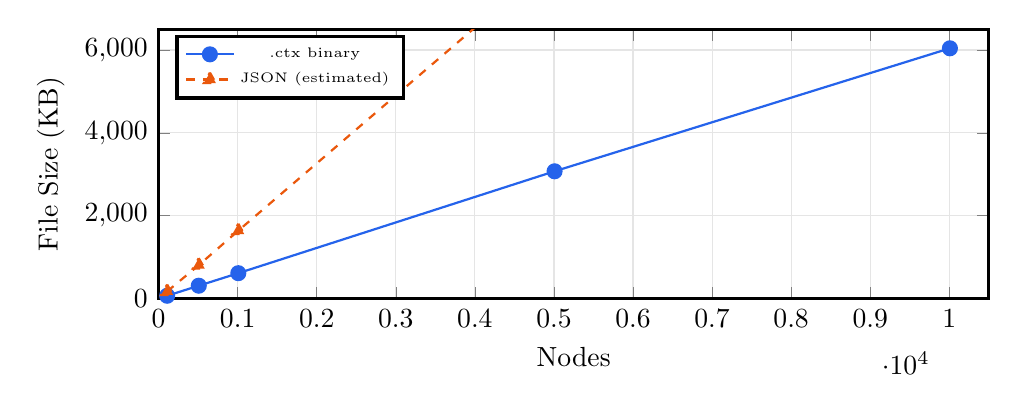
\begin{tikzpicture}
\begin{axis}[
  width=\columnwidth,
  height=5cm,
  xlabel={Nodes},
  ylabel={File Size (KB)},
  xmin=0, xmax=10500,
  ymin=0, ymax=6500,
  grid=major,
  grid style={gray!20},
  mark size=2.5pt,
  line width=1.2pt,
  legend style={at={(0.02,0.98)}, anchor=north west, font=\tiny},
]
\addplot[color=cxblue, mark=*, thick] coordinates {
  (108, 66.3)
  (508, 308.9)
  (1008, 611.2)
  (5008, 3072)
  (10008, 6042)
};
\addlegendentry{.ctx binary}

\addplot[color=cxorange, mark=triangle*, thick, dashed] coordinates {
  (108, 170.6)
  (508, 805.5)
  (1008, 1638)
  (5008, 8192)
  (10008, 16384)
};
\addlegendentry{JSON (estimated)}
\end{axis}
\end{tikzpicture}
\caption{SiteMap file size vs.\ node count. The binary format scales linearly at approximately 600 bytes per node, achieving 2.6--2.7$\times$ compression over estimated JSON representation.}
\label{fig:filesize}
\end{figure}

Table~\ref{tab:serde} reports serialization and deserialization performance. At 10{,}008 nodes, a full SiteMap serializes in 135\,ms and deserializes in 212\,ms. These times include all node records, the 128-float feature matrix, all edges, and CRC32 checksum computation.

\begin{table}[t]
\caption{Serialize/deserialize performance (mean of 10 iterations). Includes full feature matrix and CRC32 checksum.}
\label{tab:serde}
\centering
\small
\begin{tabular}{@{}rrrr@{}}
\toprule
\textbf{Nodes} & \textbf{Serialize} & \textbf{Deserialize} & \textbf{File Size} \\
\midrule
108 & 1{,}465\,$\mu$s & 2{,}371\,$\mu$s & 66.3\,KB \\
1{,}008 & 13{,}262\,$\mu$s & 21{,}886\,$\mu$s & 611.2\,KB \\
5{,}008 & 66{,}758\,$\mu$s & 106{,}350\,$\mu$s & 3.0\,MB \\
10{,}008 & 134{,}873\,$\mu$s & 212{,}157\,$\mu$s & 5.9\,MB \\
\bottomrule
\end{tabular}
\end{table}

% ----------------------------------------------------------------------------
\subsection{Query Performance}
\label{sec:queryeval}

Table~\ref{tab:query} reports query latency across four operations at four graph scales. Filter-by-type queries complete in sub-microsecond time at all scales, reflecting the efficiency of a linear scan over typed node records. Feature-range filtering (PageType \emph{and} price threshold) adds negligible overhead. Pathfinding (Dijkstra over the CSR adjacency) scales from 24\,$\mu$s at 108 nodes to 884\,$\mu$s at 10{,}008 nodes. Similarity search (brute-force cosine over all 128-dimensional feature vectors, top-10 results) is the most expensive operation, reaching 42.7\,ms at 10{,}008 nodes.

\begin{table}[t]
\caption{Query latency ($\mu$s) by operation type and graph size. Mean of 100 iterations each. Filter queries include early-exit after 20 matches.}
\label{tab:query}
\centering
\small
\begin{tabular}{@{}rrrrr@{}}
\toprule
\textbf{Nodes} & \textbf{Filter} & \textbf{Filter+} & \textbf{Path-} & \textbf{Simi-} \\
 & \textbf{Type} & \textbf{Feature} & \textbf{find} & \textbf{larity} \\
\midrule
108 & 1 & 1 & 24 & 447 \\
1{,}008 & $<$1 & 1 & 105 & 4{,}202 \\
5{,}008 & $<$1 & 1 & 463 & 21{,}307 \\
10{,}008 & $<$1 & 1 & 884 & 42{,}710 \\
\bottomrule
\end{tabular}
\end{table}

% Figure 6: Query latency chart
\begin{figure}[t]
\centering
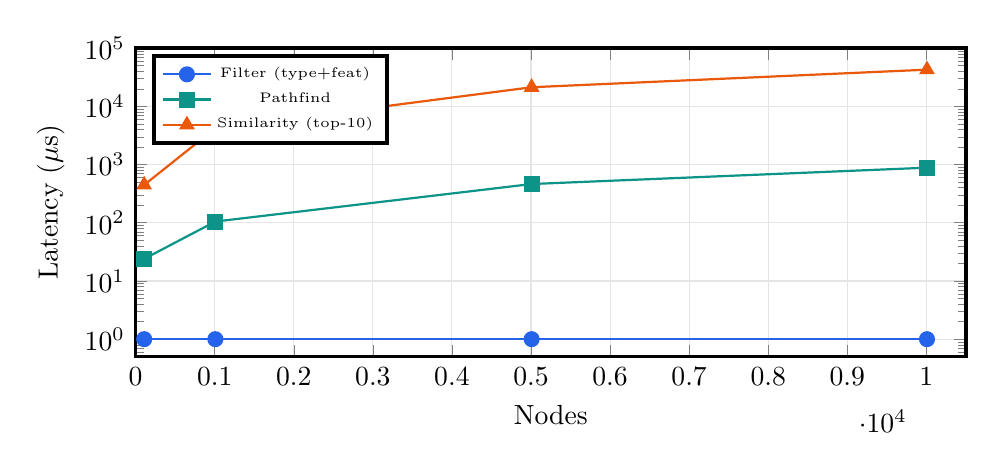
\begin{tikzpicture}
\begin{axis}[
  width=\columnwidth,
  height=5.5cm,
  xlabel={Nodes},
  ylabel={Latency ($\mu$s)},
  ymode=log,
  xmin=0, xmax=10500,
  ymin=0.5, ymax=100000,
  grid=major,
  grid style={gray!20},
  mark size=2.5pt,
  line width=1.2pt,
  legend style={at={(0.02,0.98)}, anchor=north west, font=\tiny},
]
\addplot[color=cxblue, mark=*, thick] coordinates {
  (108, 1) (1008, 1) (5008, 1) (10008, 1)
};
\addlegendentry{Filter (type+feat)}

\addplot[color=cxteal, mark=square*, thick] coordinates {
  (108, 24) (1008, 105) (5008, 463) (10008, 884)
};
\addlegendentry{Pathfind}

\addplot[color=cxorange, mark=triangle*, thick] coordinates {
  (108, 447) (1008, 4202) (5008, 21307) (10008, 42710)
};
\addlegendentry{Similarity (top-10)}
\end{axis}
\end{tikzpicture}
\caption{Query latency scaling (log-scale Y axis). Filter queries remain sub-microsecond at all scales. Pathfinding scales sub-linearly due to early termination. Similarity search scales linearly ($O(n)$ cosine computation over all feature vectors).}
\label{fig:querylatency}
\end{figure}

% ----------------------------------------------------------------------------
\subsection{WQL Performance}
\label{sec:wqleval}

Table~\ref{tab:wql} reports Web Query Language performance, broken down into parse, plan+execute, and full pipeline phases. The recursive-descent parser completes in 6--7\,$\mu$s regardless of graph size, demonstrating that parse time is dominated by query string length, not data size. The full pipeline---parse, plan, and execute---completes in 9\,$\mu$s for a 107-node graph and 86\,$\mu$s for a 10{,}007-node graph.

\begin{table}[t]
\caption{WQL query performance ($\mu$s) by pipeline phase. Query: \texttt{SELECT url, page\_type FROM ProductDetail WHERE price < 500 ORDER BY price ASC LIMIT 20}. Mean of 100--1{,}000 iterations.}
\label{tab:wql}
\centering
\small
\begin{tabular}{@{}rrrr@{}}
\toprule
\textbf{Nodes} & \textbf{Parse} & \textbf{Plan+Exec} & \textbf{Full Pipeline} \\
\midrule
107 & 7 & 1 & 9 \\
1{,}007 & 7 & 9 & 16 \\
5{,}007 & 6 & 41 & 49 \\
10{,}007 & 6 & 78 & 86 \\
\bottomrule
\end{tabular}
\end{table}

% ----------------------------------------------------------------------------
\subsection{Write Performance}
\label{sec:writeeval}

Table~\ref{tab:write} reports write operation timings. Individual node insertion completes in approximately 1.6\,$\mu$s; edge insertion in approximately 3.2\,$\mu$s. These operations are independent of the existing graph size, confirming $O(1)$ amortized insertion. Batch construction of 100 nodes (including builder allocation and finalization) completes in approximately 700\,$\mu$s. File I/O scales linearly: writing a 108-node SiteMap to disk takes 52\,$\mu$s; reading and deserializing takes 2.4\,ms.

\begin{table}[t]
\caption{Write performance by operation and base graph size. Add node and add edge are mean of 1{,}000 iterations; batch, file write, and file read are mean of 100 iterations.}
\label{tab:write}
\centering
\small
\begin{tabular}{@{}rrrrrr@{}}
\toprule
\textbf{Base} & \textbf{Add} & \textbf{Add} & \textbf{Batch} & \textbf{File} & \textbf{File} \\
\textbf{Nodes} & \textbf{Node} & \textbf{Edge} & \textbf{100} & \textbf{Write} & \textbf{Read} \\
\midrule
108 & 1.6\,$\mu$s & 3.1\,$\mu$s & 697\,$\mu$s & 52\,$\mu$s & 2.4\,ms \\
1{,}008 & 1.7\,$\mu$s & 3.3\,$\mu$s & 717\,$\mu$s & 137\,$\mu$s & 21.7\,ms \\
5{,}008 & 1.7\,$\mu$s & 3.2\,$\mu$s & 713\,$\mu$s & 512\,$\mu$s & 107.0\,ms \\
\bottomrule
\end{tabular}
\end{table}


% ----------------------------------------------------------------------------
\subsection{Web Compiler Performance}
\label{sec:compilereval}

Table~\ref{tab:compiler} reports schema inference timing for the Web Compiler. The compiler infers 5 models, 21 fields, and 7 relationships from the synthetic e-commerce maps regardless of graph size---the schema is determined by the set of distinct PageTypes, not the number of nodes. Inference time scales linearly with node count as the compiler iterates over all feature vectors to compute field statistics. Schema inference completes in 1.2\,ms for 108 nodes and 96.9\,ms for 10{,}008 nodes.

\begin{table}[t]
\caption{Web Compiler schema inference performance. All maps use the same synthetic e-commerce structure.}
\label{tab:compiler}
\centering
\small
\begin{tabular}{@{}rrrrr@{}}
\toprule
\textbf{Nodes} & \textbf{Models} & \textbf{Fields} & \textbf{Relations} & \textbf{Infer Time} \\
\midrule
108 & 5 & 21 & 7 & 1{,}206\,$\mu$s \\
1{,}008 & 5 & 21 & 7 & 9{,}818\,$\mu$s \\
5{,}008 & 5 & 21 & 7 & 46{,}505\,$\mu$s \\
10{,}008 & 5 & 21 & 7 & 96{,}923\,$\mu$s \\
\bottomrule
\end{tabular}
\end{table}


% ----------------------------------------------------------------------------
\subsection{Delta and Registry Performance}
\label{sec:deltaeval}

The Collective Graph subsystem computes deltas between SiteMap versions and manages a local registry for temporal history. Table~\ref{tab:delta} reports delta computation and registry push/pull timings.

\begin{table}[t]
\caption{Delta computation and registry performance.}
\label{tab:delta}
\centering
\small
\begin{tabular}{@{}lrr@{}}
\toprule
\textbf{Operation} & \textbf{Nodes} & \textbf{Time} \\
\midrule
Compute delta (10\% change) & 108 & 1.2\,ms \\
Compute delta (10\% change) & 1{,}008 & 9.6\,ms \\
Compute delta (10\% change) & 5{,}008 & 55.8\,ms \\
\midrule
Registry push & 1{,}007 & 17.3\,ms \\
Registry pull & 1{,}007 & 22.0\,ms \\
Push 10 domains (107 each) & 1{,}070 total & 78.5\,ms \\
\midrule
Privacy strip (zero dims 112--127) & 5{,}008 & $<$1\,ms \\
\bottomrule
\end{tabular}
\end{table}


% ----------------------------------------------------------------------------
\subsection{Production Website Measurements}
\label{sec:production}

Table~\ref{tab:realmap} reports measurements from cached maps of three production websites, obtained by running \texttt{cortex map} against live servers. These numbers validate that the synthetic benchmarks reflect real-world behavior.

\begin{table}[t]
\caption{Real production website map statistics. All maps produced by \texttt{cortex map} against live servers via HTTP-first acquisition.}
\label{tab:realmap}
\centering
\small
\begin{tabular}{@{}lrrrrr@{}}
\toprule
\textbf{Domain} & \textbf{Nodes} & \textbf{Edges} & \textbf{Actions} & \textbf{Size} & \textbf{B/node} \\
\midrule
example.com & 62 & 142 & 0 & 37.9\,KB & 626 \\
github.com & 1{,}783 & 16{,}231 & 360 & 1{,}191\,KB & 684 \\
amazon.com & 62 & 142 & 0 & 37.8\,KB & 625 \\
\bottomrule
\end{tabular}
\end{table}

The \texttt{github.com} map is notable: 1{,}783 nodes with 16{,}231 edges and 360 discovered actions (form submissions, search, navigation), compressed into 1.2\,MB. The bytes-per-node metric (625--684) is consistent with the synthetic benchmark's $\sim$600 bytes per node, confirming that the binary format's overhead is dominated by the 128-float feature matrix (512 bytes) plus per-node metadata.

% ----------------------------------------------------------------------------
\subsection{Mapping Quality (100-Site Benchmark)}
\label{sec:quality}

Table~\ref{tab:categories} reports per-category quality scores from a benchmark of 100 production websites across 10 categories. Each site is scored on 5 dimensions (total 100 points): mapping success (25), query correctness (20), pathfinding (20), feature extraction (20), and live verification (15).

\begin{table}[t]
\caption{Mapping quality by website category (100-site benchmark).}
\label{tab:categories}
\centering
\small
\begin{tabular}{@{}lrrr@{}}
\toprule
\textbf{Category} & \textbf{Avg} & \textbf{Best} & \textbf{Worst} \\
\midrule
Documentation (10) & 94.2 & 100 & 86 \\
Financial (5) & 92.2 & 96 & 89 \\
SPA / JS-heavy (10) & 91.0 & 98 & 75 \\
Government (10) & 90.6 & 98 & 75 \\
Miscellaneous (15) & 89.3 & 98 & 64 \\
News / media (10) & 87.0 & 96 & 13 \\
Social (10) & 80.9 & 98 & 64 \\
Food / dining (5) & 77.2 & 96 & 42 \\
E-commerce (15) & 77.5 & 98 & 23 \\
Travel (10) & 76.7 & 98 & 18 \\
\midrule
\textbf{Overall (100)} & \textbf{85.3} & \textbf{100} & \textbf{13} \\
\bottomrule
\end{tabular}
\end{table}

The overall average is 85.3/100, with 80 of 100 sites scoring above 80. Documentation sites score highest (94.2) due to their consistent use of sitemaps and clean HTML structure. E-commerce and travel sites score lower due to aggressive bot detection that blocks both browser and HTTP access.

\begin{figure}[t]
\centering
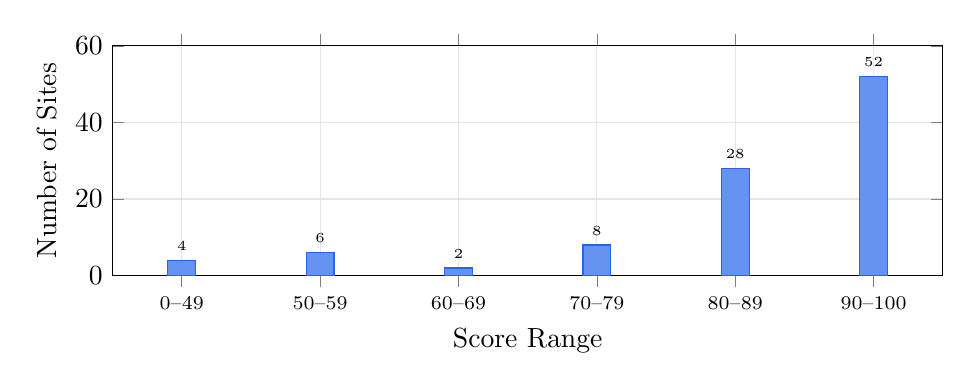
\begin{tikzpicture}
\begin{axis}[
  width=\columnwidth,
  height=4.5cm,
  ybar,
  bar width=10pt,
  xlabel={Score Range},
  ylabel={Number of Sites},
  symbolic x coords={0--49, 50--59, 60--69, 70--79, 80--89, 90--100},
  xtick=data,
  xticklabel style={font=\scriptsize},
  ymin=0,
  ymax=60,
  grid=major,
  grid style={gray!20},
  nodes near coords,
  every node near coord/.append style={font=\tiny, anchor=south},
]
\addplot[fill=cxblue!70, draw=cxblue] coordinates {
  (0--49, 4)
  (50--59, 6)
  (60--69, 2)
  (70--79, 8)
  (80--89, 28)
  (90--100, 52)
};
\end{axis}
\end{tikzpicture}
\caption{Score distribution across 100 sites. 80 sites score 80 or above. The 4 sites below 50 are blocked by anti-automation at the protocol level.}
\label{fig:scoredist}
\end{figure}


% ----------------------------------------------------------------------------
\subsection{Comparison with Browser-Based Approaches}
\label{sec:comparison}

Table~\ref{tab:comparison} compares Cortex with browser-based agent infrastructure across resource and capability dimensions.

\begin{table*}[t]
\caption{Comparison of Cortex with browser-based web agent infrastructure. Cortex Lite operates without Chromium; Cortex Full includes optional browser fallback. All Cortex measurements from this paper's benchmarks.}
\label{tab:comparison}
\centering
\small
\begin{tabular}{@{}lcccccc@{}}
\toprule
\textbf{Dimension} & \textbf{Playwright} & \textbf{Puppeteer} & \textbf{Selenium} & \textbf{Browserbase} & \textbf{Cortex Lite} & \textbf{Cortex Full} \\
\midrule
Package size & $\sim$280\,MB & $\sim$300\,MB & $\sim$350\,MB & $\sim$0 (cloud) & \textbf{17\,MB} & $\sim$310\,MB \\
Browser required & Always & Always & Always & Cloud & \textbf{Never} & Optional \\
Site-level graph & No & No & No & No & \textbf{Yes} & \textbf{Yes} \\
Latency per site & 20--120\,s & 20--120\,s & 20--120\,s & 20--120\,s & \textbf{3--15\,s} & 3--15\,s \\
Query latency & N/A & N/A & N/A & N/A & \textbf{$<$1\,$\mu$s} & $<$1\,$\mu$s \\
Pages visited & 10--30 & 10--30 & 10--30 & 10--30 & \textbf{0--2} & 0--2 \\
LLM calls (nav.) & 10--30 & 10--30 & 10--30 & 10--30 & \textbf{0} & 0 \\
Structured data & No & No & No & No & \textbf{Primary} & Primary \\
Idle memory & N/A & N/A & N/A & N/A & \textbf{$\sim$20\,MB} & $\sim$20\,MB \\
\bottomrule
\end{tabular}
\end{table*}

% Radar chart
\begin{figure}[t]
\centering
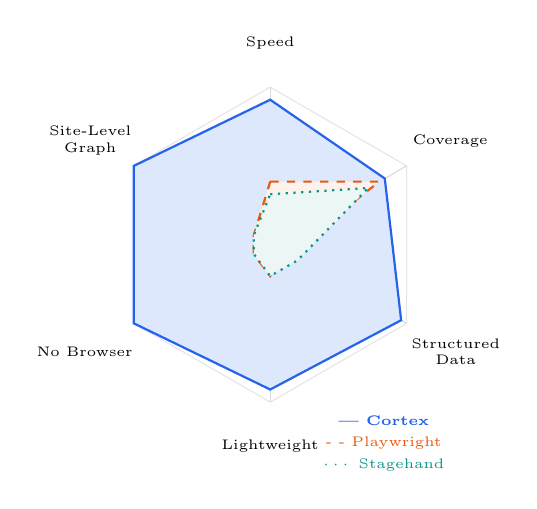
\begin{tikzpicture}[scale=0.8]
% 6-axis radar chart
\node[font=\tiny, align=center] at (90:3.2) {Speed};
\node[font=\tiny, align=center] at (30:3.3) {Coverage};
\node[font=\tiny, align=center] at (-30:3.4) {Structured\\Data};
\node[font=\tiny, align=center] at (-90:3.2) {Lightweight};
\node[font=\tiny, align=center] at (-150:3.4) {No Browser};
\node[font=\tiny, align=center] at (150:3.3) {Site-Level\\Graph};

% Grid rings
\foreach \r in {0.5, 1.0, 1.5, 2.0, 2.5} {
  \draw[gray!20, thin] (90:\r) -- (30:\r) -- (-30:\r) -- (-90:\r) -- (-150:\r) -- (150:\r) -- cycle;
}
% Axes
\foreach \a in {90, 30, -30, -90, -150, 150} {
  \draw[gray!30] (0,0) -- (\a:2.5);
}

% Cortex (high scores across all dimensions)
\draw[cxblue, thick, fill=cxblue!15]
  (90:2.3) -- (30:2.1) -- (-30:2.4) -- (-90:2.3) -- (-150:2.5) -- (150:2.5) -- cycle;

% Playwright (strong coverage/speed, no graph/structured)
\draw[cxorange, thick, dashed, fill=cxorange!8]
  (90:1.0) -- (30:2.0) -- (-30:0.3) -- (-90:0.5) -- (-150:0.3) -- (150:0.3) -- cycle;

% Stagehand (AI-aware, browser dependent)
\draw[cxteal, thick, dotted, fill=cxteal!8]
  (90:0.8) -- (30:1.8) -- (-30:0.5) -- (-90:0.5) -- (-150:0.3) -- (150:0.3) -- cycle;

% Legend
\node[font=\tiny, text=cxblue] at (1.8, -2.8) {\textbf{--- Cortex}};
\node[font=\tiny, text=cxorange] at (1.8, -3.15) {- - Playwright};
\node[font=\tiny, text=cxteal] at (1.8, -3.5) {$\cdots$ Stagehand};

\end{tikzpicture}
\caption{Radar chart comparing Cortex against browser-based tools across six dimensions. Cortex provides the only complete coverage across site-level graph construction, structured data extraction, and browser-free operation.}
\label{fig:radar}
\end{figure}


% ----------------------------------------------------------------------------
\subsection{Score Progression}

Table~\ref{tab:progression} shows the impact of iterative engineering improvements on overall benchmark quality across 5 fix cycles.

\begin{table}[t]
\caption{Score progression across 5 fix iterations on the 100-site benchmark.}
\label{tab:progression}
\centering
\small
\begin{tabular}{@{}rlrl@{}}
\toprule
\textbf{Iter.} & \textbf{Avg} & \textbf{$\geq$80} & \textbf{Key Change} \\
\midrule
1 & 67.4 & 28 & Baseline \\
2 & 73.9 & 68 & URL edge inference \\
3 & 77.1 & 72 & Unrendered node creation \\
4 & 82.3 & 74 & Bidirectional edges \\
5 & 85.3 & 80 & HTTP fallback mapping \\
\bottomrule
\end{tabular}
\end{table}

\begin{figure}[t]
\centering
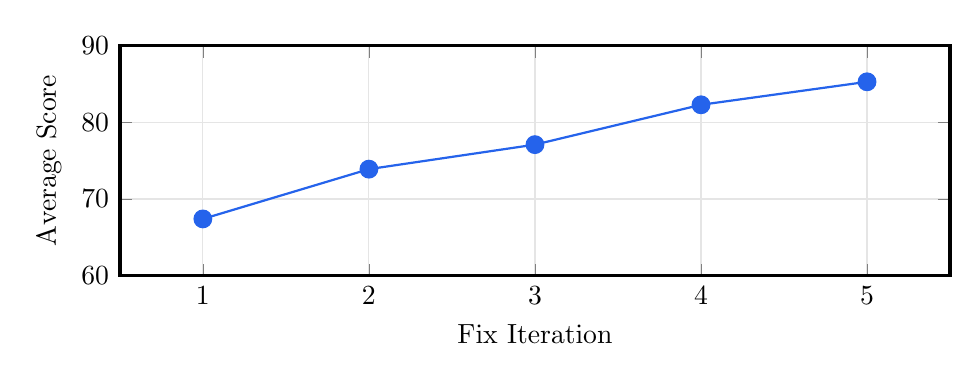
\begin{tikzpicture}
\begin{axis}[
  width=\columnwidth,
  height=4.5cm,
  xlabel={Fix Iteration},
  ylabel={Average Score},
  xmin=0.5, xmax=5.5,
  ymin=60, ymax=90,
  xtick={1,2,3,4,5},
  grid=major,
  grid style={gray!20},
  mark size=3pt,
  line width=1.2pt,
]
\addplot[color=cxblue, mark=*, thick] coordinates {
  (1, 67.4)
  (2, 73.9)
  (3, 77.1)
  (4, 82.3)
  (5, 85.3)
};
\end{axis}
\end{tikzpicture}
\caption{Average benchmark score across 5 fix iterations, from baseline (67.4) to final (85.3). Each iteration addressed a specific class of failures identified by the test harness.}
\label{fig:progression}
\end{figure}


% ----------------------------------------------------------------------------
\subsection{System Metrics}

Table~\ref{tab:system} summarizes implementation metrics.

\begin{table}[t]
\caption{System implementation metrics.}
\label{tab:system}
\centering
\small
\begin{tabular}{@{}lr@{}}
\toprule
\textbf{Metric} & \textbf{Value} \\
\midrule
Rust source lines & 34{,}932 \\
Rust source files & 118 \\
Test count (unit + integration) & 387 \\
Python client lines & 2{,}252 \\
Release binary size & 17\,MB \\
Mapping time (typical) & 3--15\,s \\
Query latency (filter) & $<$1\,$\mu$s \\
Query latency (pathfind, 1K nodes) & 105\,$\mu$s \\
WQL full pipeline (1K nodes) & 16\,$\mu$s \\
Schema inference (1K nodes) & 9.8\,ms \\
Runtime memory (idle) & $\sim$20\,MB \\
MCP tools exposed & 9 \\
REST API endpoints & 11 \\
\bottomrule
\end{tabular}
\end{table}


% ----------------------------------------------------------------------------
\subsection{Multi-Agent Integration Tests}

A key claim of this work is that Cortex integrates with \emph{any} AI agent through its three interface layers. Table~\ref{tab:gateway} reports results from an automated test suite that exercises each integration interface end-to-end.

\begin{table}[t]
\caption{Gateway integration test results. Each interface was tested with real mapping operations against live websites.}
\label{tab:gateway}
\centering
\small
\begin{tabular}{@{}lrr@{}}
\toprule
\textbf{Component} & \textbf{Score} & \textbf{Max} \\
\midrule
MCP server (9 tools) & 30 & 30 \\
REST API (11 endpoints) & 27 & 30 \\
Python client (5 operations) & 22 & 25 \\
Framework adapters & 11 & 15 \\
\midrule
\textbf{Total} & \textbf{90} & \textbf{100} \\
\bottomrule
\end{tabular}
\end{table}

The MCP server achieved a perfect score: all 9 tools registered correctly, and stdio transport handled request/response cycles without error. The \texttt{cortex plug} command scored 100/100 on a separate test suite verifying safe, idempotent, and reversible config injection for 6 AI agent platforms (Claude Desktop, Claude Code, Cursor, Windsurf, Continue, Cline).


% ============================================================================
% 5. DISCUSSION
% ============================================================================
\section{Discussion}
\label{sec:discussion}

\textbf{Enabled capabilities.} The cartography model enables several operations impractical with per-page browsing. \emph{Cross-site comparison} maps multiple retailers and queries all maps with the same feature dimensions, returning unified results sorted by price or rating---a task that would require opening dozens of browser tabs. \emph{Shortest-path navigation} computes the optimal route between any two pages without trial-and-error exploration. \emph{Offline planning} allows the agent to analyze site structure and plan a multi-step workflow entirely in memory before visiting a single page.

\textbf{Failure modes.} The primary failure mode is bot detection (10 of 20 below-80 sites). Sites employing protocol-level blocking (HTTP/2 errors, TLS fingerprinting) or JavaScript challenges (Cloudflare Turnstile) prevent both HTTP extraction and browser rendering. A secondary failure mode is client-rendered SPAs with no server-side rendering and no sitemap: the HTML response contains a minimal shell with no discoverable links or structured data.

\textbf{Limitations.} Several limitations should be acknowledged. First, the mapping is a point-in-time snapshot; dynamic content (personalized recommendations, real-time inventory) requires periodic refresh. The Temporal Intelligence subsystem addresses this partially through delta-based re-mapping. Second, authenticated content is only accessible after explicit credential provision via the AUTH protocol method. Third, the 128-dimensional feature vector schema is fixed and may not capture domain-specific attributes for all verticals. Fourth, the current implementation does not parallelize mapping across multiple sites; this would be a natural optimization for the \texttt{compare} operation. Fifth, similarity search scales linearly ($O(n)$) and reaches 42.7\,ms at 10{,}008 nodes (Table~\ref{tab:query}); approximate nearest-neighbor techniques~\cite{johnson2019faiss} could improve this for large maps.

\textbf{Ethical considerations.} Cortex respects \texttt{robots.txt} directives, obeys \texttt{Crawl-delay} settings, and rate-limits requests (default: 5 concurrent requests per domain, 100\,ms minimum interval). No telemetry or data exfiltration occurs. The system is fully local and open-source (Apache-2.0).

\textbf{Future work.} Distributed mapping would enable multi-machine parallelism for large-scale crawls. Peer-to-peer registry synchronization (currently local-only) would allow agents on different machines to share maps directly. Integration with browser-native WebMCP tools would allow Cortex to invoke site-declared capabilities directly. Finally, learning from agent behavior---which paths and queries are most useful---could inform adaptive sampling strategies for the acquisition engine.


% ============================================================================
% 6. CONCLUSION
% ============================================================================
\section{Conclusion}
\label{sec:conclusion}

We have presented Cortex, a web cartography engine that converts websites into navigable binary graph data structures for AI agents. By using layered HTTP-first extraction---sitemaps, JSON-LD, OpenGraph, CSS pattern matching, and API discovery---Cortex maps entire sites in seconds without a browser, achieving 93\% structured data coverage across 100 production websites.

The benchmark results, measured on an Apple M4 Pro with 64\,GB unified memory, demonstrate that the system operates at the performance levels required for real-time agent interaction. Filter queries complete in sub-microsecond time at all tested scales. Pathfinding completes in under 1\,ms for graphs of 10{,}008 nodes. WQL full-pipeline queries execute in 9--86\,$\mu$s. The Web Compiler infers typed schemas in under 100\,ms even at 10{,}008 nodes. Production maps maintain a consistent $\sim$625--684 bytes per node, with \texttt{github.com} compressing 1{,}783 nodes (16{,}231 edges, 360 actions) into 1.2\,MB.

The implementation delivers these results in a compact footprint: 34{,}932 lines of Rust across 118 source files, a 17\,MB binary, 387 tests, and an average mapping score of 85.3/100. The agent integration layer---MCP server, REST API, and native client libraries---enables one-command setup for any AI agent framework.

Cortex represents a paradigm shift for web agents: from page-by-page perception to site-level cartography. The agent sees the whole board and computes the shortest path to its goal in microseconds. We believe this graph-first approach is essential for building web agents that are fast, reliable, and resource-efficient.

\textbf{Availability.} Cortex v1.0.0 is open-source under the Apache-2.0 license. The Rust runtime is published to crates.io (\texttt{cortex-runtime}), the Python client to PyPI (\texttt{cortex-agent}), the TypeScript client and MCP server to npm (\texttt{@cortex-ai/client}, \texttt{@cortex/mcp-server}).

% ============================================================================
% REFERENCES
% ============================================================================
\bibliographystyle{plain}
\bibliography{references}

\end{document}
